\documentclass{standalone}
\usepackage{tikz}
\usetikzlibrary{arrows.meta}

\begin{document}

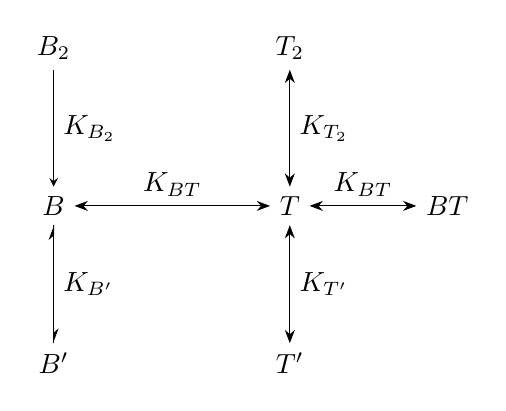
\begin{tikzpicture}[auto, node distance=2cm, >=Stealth]

    % Nodes
    \node (B2) {$B_2$};
    \node (B) [below of=B2] {$B$};
    \node (B') [below of=B] {$B'$};
    \node (T2) [right of=B2, node distance=3cm] {$T_2$};
    \node (T) [below of=T2] {$T$};
    \node (T') [below of=T] {$T'$};
    \node (BT) [right of=T, node distance=2cm] {$BT$};
    
    % Arrows
    \draw[->, >=stealth] (B2) to node {$K_{B_2}$} (B);
    \draw[arrows = {-Stealth[harpoon]}] (B) to node {$K_{B'}$} (B');
    \draw[arrows = {-Stealth[harpoon]}] (B') to node  {} (B);
    \draw[<->] (T2) to node {$K_{T_2}$} (T);
    \draw[<->] (T) to node {$K_{T'}$} (T');
    \draw[<->] (B) to node {$K_{BT}$} (T);
    \draw[<->] (T) to node {$K_{BT}$} (BT);
\end{tikzpicture}

\end{document}
